\documentclass{article}

% === Input and Encoding ===
\usepackage[utf8]{inputenc}
\DeclareUnicodeCharacter{FFFD}{} % Avoid Unicode errors

% === Essential Packages ===
\usepackage{graphicx}
\usepackage{caption}
\usepackage{subcaption}
\usepackage{float}
\usepackage{adjustbox}
\usepackage{tikz}
\usepackage{listings}
\usepackage{xcolor}
\usepackage{siunitx}
\usepackage{amsmath, amssymb, amsthm}
\usepackage{setspace}
\usepackage{verbatim}
\usepackage{tocloft}
\usepackage{pdfpages}

% === URL Handling ===
\usepackage{xurl} % Better URL line breaking
\Urlmuskip=0mu plus 1mu
\sloppy % More forgiving line breaking

% === Hyperlinks ===
\usepackage{hyperref}
\hypersetup{
  colorlinks=true,
  linkcolor=blue,
  citecolor=blue,
  urlcolor=blue
}

% === Bibliography: Cambridge-style Author–Date ===
\usepackage[
  backend=biber,
  style=authoryear,
  citestyle=authoryear,
  maxcitenames=2,
  maxbibnames=99,
  doi=false,
  isbn=false,
  url=false
]{biblatex}
\addbibresource{references.bib}
\setlength\bibitemsep{1.5\itemsep}

% === Code Listings Configuration ===
\lstset{
  language=Python,
  basicstyle=\ttfamily\footnotesize,
  keywordstyle=\color{blue},
  commentstyle=\color{gray},
  stringstyle=\color{green!50!black},
  showstringspaces=false,
  breaklines=true,
  frame=single,
  tabsize=2,
  captionpos=b
}

% === TikZ Libraries ===
\usetikzlibrary{
  positioning,
  shapes.geometric,
  arrows.meta,
  calc,
  3d,
  backgrounds,
  shadows,
  shadows.blur,
  shapes.multipart
}

% === Word Count (Optional for Local Use) ===
\immediate\write18{texcount -1 -sum=1 -utf8 \jobname.tex > \jobname.wordcount}
\newcommand\wordcount{\verbatiminput{\jobname.wordcount}}







\begin{document}
\sloppy
\begin{titlepage}
    \begin{center}
        \vspace*{1cm}
        \includegraphics[width=0.45\textwidth]{latexImage_af6761d75bc1259f2c1d15bd34be3b35.png}
        \hfill
        \includegraphics[width=0.45\textwidth]{latexImage_e05fa6d9de397203e740a37265984f2e.png}
        
        \vspace{1.5cm}
        \LARGE \textbf{MSc Data Analytics and Technologies}
        
        \vspace{1.5cm}
        \Large CDM7102
        
        \vspace{0.5cm}
        \textbf{Grape Farming and Wine Making: A Data-Driven Approach}
        
        \vspace{0.5cm}
        Assessment: 001 Portfolio
        
        \vfill
        \textbf{Module Tutor:} \\
        Dr. George Prokopakis
        
        \vspace{0.8cm}
        \textbf{Student ID:} \\
        100-0089131
        
        \vspace{0.8cm}
        \textbf{May 2025}
        
        \vspace{0.8cm}
        Word count: 10066       
        \vfill
    \end{center}
\end{titlepage}





\sloppy



\newpage
\tableofcontents
\newpage
\doublespacing

\section{Introduction}
\subsection{Background}


The convergence of precision agriculture, machine learning, and Internet of Things (IoT) technologies has transformed traditional viticulture into a data-driven discipline. Historically, vineyard management relied on tacit knowledge, manual observations, and seasonal heuristics for critical decisions regarding irrigation, pruning, pest control, and harvest timing \parencite{jackson2020wine}. However, increased climate variability and the demand for high-quality, traceable wine production have necessitated more accurate, timely, and location-specific insights \parencite{gladstones2011wine, jones2007climate}.

Modern precision viticulture integrates environmental sensing, cloud-based analytics, and predictive modeling to optimize grapevine performance while minimizing resource usage \parencite{kamilaris2018deep, zhang2022iot}. Real-time data acquisition from sensors and weather APIs offers detailed insights into microclimatic dynamics, while machine learning algorithms identify patterns and predict outcomes including grape maturity, disease risk, and optimal harvest windows \parencite{ratnaparkhi2021review}.

Recent advances in edge computing have enabled these models to be deployed on low-power devices like Raspberry Pi, facilitating in-field analytics without the need for continuous cloud connectivity \parencite{liu2020edge, alazab2021raspberry}. This has opened opportunities for scalable deployment in small and medium-sized vineyards, particularly in geographically diverse wine regions like Greece, where local microclimates critically influence grape composition and sensory profiles \parencite{white2009soil, vanleeuwen2016impact}.

To bridge the gap between advanced modeling and vineyard operations, interactive dashboards built with Streamlit offer an intuitive interface for stakeholders. They enable growers to visualize predictions, compare regions, and download insights in real time \parencite{fan2021streamlit, BaltzakisThemistoklis2025streamlit}. When paired with backend frameworks like Apache Airflow and FastAPI, these tools create a practical, scalable smart viticulture system.

This research builds on these foundations by utilizing a vineyard analytics pipeline that integrates weather forecasting, time series modeling, and user-friendly dashboards to support evidence-based decisions in grape farming.

\addcontentsline{toc}{section}{Executive Summary}

This dissertation explores how data analytics can transform grape cultivation and wine-making practices in Greek vineyards. By analyzing real-world climate data—including temperature, humidity, and precipitation—it investigates how environmental conditions affect grape quality and viticultural success \cite{jackson2020wine, jones2007climate, koundouras2006influence}. Emphasis is placed on exploratory data analysis (EDA) and time series forecasting, with temperature identified as a critical factor in grape ripening and sugar development \cite{gladstones2011wine, vanleeuwen2016impact}.

The study evaluates environmental datasets from six key Greek wine regions, using statistical metrics like mean, variance, and range to highlight regional microclimate differences \cite{white2009soil, koundouras1999response}. These insights support adaptive farming practices. Forecasting models assess trends in temperature and humidity and identify risks such as heatwaves and early frost events \cite{smith2021forecasting, zhang2022iot, zerefos2014climate}.

To enhance decision-making, the research integrates Internet of Things (IoT) sensors and machine learning techniques for predictive vineyard management \cite{sharma2020iot, kamilaris2018deep}. These tools enable smarter irrigation and harvest planning, helping maintain grape consistency, optimize resource usage, and increase climate resilience in viticulture \cite{cozzolino2011role, lobell2008climate, panagos2022climate}.

A publicly accessible, interactive dashboard was created to showcase the system’s practical application. This tool visualizes real-time environmental forecasts and supports data-driven decision-making at the vineyard level. It can be accessed at: \href{https://xgboost-forecasting.streamlit.app}{xgboost-forecasting.streamlit.app} \cite{BaltzakisThemistoklis2025streamlit}.




  
\subsection{Motivation and Significance}

Although publicly available meteorological datasets and environmental sensors exist, many vineyards in Greece still rely on traditional methods and often lack the analytical capabilities to interpret complex environmental signals effectively. Regions with stable microclimates, like Siteia and Santorini, may benefit from predictive irrigation and harvest scheduling \parencite{white2009soil}, while vineyards in areas with greater temperature fluctuations, such as Koropi and Amyntaio, require more adaptive strategies. The limited use of machine learning, exploratory data analysis (EDA), and time series forecasting has resulted in the underutilization of valuable data assets \parencite{zhang2022iot, smith2021forecasting}.

This dissertation addresses the gap by using a data-driven framework to evaluate historical environmental conditions across six major Greek viticultural regions: Amyntaio, Archanes, Heraklion, Koropi, Santorini, and Siteia. Through descriptive statistics, correlation analysis, and time series forecasting, it offers growers practical decision-support tools to enhance yield, consistency, and sustainability.

Despite Greece’s rich enological tradition, regional wineries face increasing climate-related risks, including heatwaves, droughts, and irregular precipitation patterns \parencite{jones2007climate, zerefos2014climate}. These changes significantly influence grape ripening stages, sugar concentration (°Brix), acidity levels, and phenolic development—key traits that determine wine quality and market value \parencite{gladstones2011wine, jackson2020wine}. Microclimatic variation in Greek vineyards—especially due to differences in elevation and maritime exposure—strongly affects grape physiology and wine typicity \parencite{koundouras2006influence, kotseridis2006wine}.

In particular, the works of Greek scholars Koundouras and Kotseridis emphasize the nuanced interaction between soil, climate, and grapevine response in regions like Nemea and Northern Greece \parencite{koundouras1999response}. Additionally, books such as *Greek Wine: A New Era* by Stavrakakis \parencite{stavrakakis2013greek} and *Climate and Viticulture in the Eastern Mediterranean* by Zerefos and Retalis \parencite{zerefos2012climatebook} contextualize the unique climatic dynamics that define viticulture in Greece.

As Greek vineyards face global competition, sustainability challenges, and environmental uncertainty, it is essential to blend traditional viticultural knowledge with modern technologies—particularly sensor networks, cloud platforms, and machine learning—to create scalable, climate-resilient vineyard strategies.


\subsection{Aims and Objectives}

The primary aim of this study is to examine how data analytics, including exploratory data analysis (EDA), time series modeling, and machine learning, can enhance viticulture in Greece. By leveraging environmental and production-related data from key vineyard regions (Amyntaio, Archanes, Heraklion, Koropi, Santorini, and Siteia), the research seeks to provide actionable insights that support more precise, adaptive, and climate-resilient vineyard management.

This investigation responds to the rising demand for precision agriculture systems that mitigate the impacts of climatic variability and shifting seasonal cycles on grapevine physiology \parencite{jones2007climate, vanleeuwen2016impact, zerefos2012climatebook}. Combining established viticultural knowledge with advanced digital technologies—such as sensor-based Internet of Things (IoT) platforms and cloud-driven analytics—can enhance decision-making related to irrigation, pruning, pest control, and harvesting \parencite{zhang2022iot, smith2021forecasting, stavrakakis2013greek}.

\begin{figure}[H]
\centering
\resizebox{0.92\textwidth}{!}{%
\begin{tikzpicture}[
  node distance=1.5cm and 2cm,
  font=\sffamily\small,
  aim/.style={
    draw,
    fill=blue!15,
    minimum width=7cm,
    minimum height=1.2cm,
    align=center,
    rounded corners,
    blur shadow
  },
  process/.style={
    draw,
    fill=orange!20,
    minimum width=5.5cm,
    minimum height=1.2cm,
    align=center,
    rounded corners,
    blur shadow
  },
  outcome/.style={
    draw,
    fill=green!25,
    minimum width=6cm,
    minimum height=1.2cm,
    align=center,
    rounded corners,
    blur shadow
  },
  arrow/.style={->, thick, >=stealth}
]

% Main aim
\node[aim] (main) {\textbf{Aim:} Use data analytics to enhance viticulture in Greece};

% Methods
\node[process, below left=1.7cm and 3.2cm of main] (eda) {�� Exploratory Data Analysis (EDA)};
\node[process, below=of main] (ts) {�� Time Series Modeling};
\node[process, below right=1.7cm and 3.2cm of main] (ml) {�� Machine Learning};

% Outcomes
\node[outcome, below=2.2cm of ts] (outcome) {Precision, adaptive, and climate-resilient vineyard management};

% Arrows
\draw[arrow] (main) -- (eda);
\draw[arrow] (main) -- (ts);
\draw[arrow] (main) -- (ml);

\draw[arrow] (eda) -- (outcome);
\draw[arrow] (ts) -- (outcome);
\draw[arrow] (ml) -- (outcome);

\end{tikzpicture}
}
\caption{Study aim and key analytical methods leading to climate-resilient vineyard management.}
\label{fig:aims-objectives-diagram}
\end{figure}




\textbf{The specific objectives of this research are as follows:}
\begin{itemize}
  \item To perform a comprehensive exploratory data analysis (EDA) of key environmental variables—temperature, humidity, and rainfall—across six major vineyard zones in Greece.
  \item To compute and interpret descriptive statistics that reveal spatial and temporal variation in climatic conditions and to visualize how these affect grapevine development and sugar accumulation \parencite{jackson2020wine, gladstones2011wine}.
  \item To implement time series forecasting models to predict short- and medium-term viticultural metrics and identify risks such as extreme heat events, frost, or prolonged drought.
  \item To conduct a comparative analysis of microclimates across the vineyard sites and determine their influence on grape yield, acidity, ripening cycles, and overall wine quality \parencite{koundouras2006influence}.
  \item To propose a reproducible, data-driven framework that integrates sensor data, climatic analytics, and machine learning techniques for use in smart viticulture applications \parencite{cozzolino2011role, kamilaris2018deep}.
\end{itemize}


\subsection{Research Questions and Hypotheses}

This study explores the intersection of environmental variability and digital technologies in grape cultivation and wine production, focusing on key vineyard regions in Greece. By integrating meteorological data, IoT-based sensing, and predictive modeling, the research aims to understand and forecast viticultural outcomes across diverse microclimates.

To guide the investigation, the following research questions (RQs) and hypotheses (Hs) are formulated:

\subsubsection*{Research Questions}

\begin{enumerate}
    \item \textbf{RQ1:} How do environmental variables such as temperature, humidity, and precipitation differ across Greek vineyard regions, and to what extent do these differences influence grape ripening and wine quality? \parencite{jackson2020wine, vanleeuwen2016impact}
    
    \item \textbf{RQ2:} In what ways can exploratory data analysis (EDA) and time series forecasting models enhance the precision and reliability of vineyard operations, such as irrigation and harvest scheduling? \parencite{jones2007climate, smith2021forecasting}
    
    \item \textbf{RQ3:} How effectively can machine learning algorithms predict viticultural indicators (e.g., sugar content, °Brix, yield) using historical climate data and sensor inputs? \parencite{kamilaris2018deep, cozzolino2011role}
    
    \item \textbf{RQ4:} What is the role of IoT-enabled monitoring systems in enabling timely, site-specific decision-making in Greek viticulture, especially under conditions of environmental uncertainty? \parencite{sharma2020iot, zhang2022iot}
\end{enumerate}

\begin{figure}[H]
\centering
\resizebox{0.95\textwidth}{!}{%
\begin{tikzpicture}[
  node distance=1.5cm and 2cm,
  font=\sffamily\small,
  question/.style={
    draw,
    fill=blue!15,
    minimum width=7.5cm,
    minimum height=1.2cm,
    align=left,
    rounded corners,
    blur shadow
  },
  method/.style={
    draw,
    fill=orange!20,
    minimum width=4.5cm,
    minimum height=1.1cm,
    align=center,
    rounded corners,
    blur shadow
  },
  arrow/.style={->, thick, >=stealth}
]

% Questions
\node[question] (rq1) {\textbf{RQ1:} How do environmental variables differ across Greek vineyard regions, and how do they influence grape ripening and wine quality?};
\node[question, below=of rq1] (rq2) {\textbf{RQ2:} How can EDA and time series forecasting improve irrigation and harvest scheduling?};
\node[question, below=of rq2] (rq3) {\textbf{RQ3:} How effectively can machine learning predict grape quality indicators (e.g., °Brix, yield)?};
\node[question, below=of rq3] (rq4) {\textbf{RQ4:} What is the role of IoT monitoring in site-specific, timely vineyard decisions?};

% Methods
\node[method, right=of rq1, xshift=4.5cm] (stat) {Statistical Analysis};
\node[method, right=of rq2, xshift=4.5cm] (ts) {Time Series Modeling};
\node[method, right=of rq3, xshift=4.5cm] (ml) {Machine Learning};
\node[method, right=of rq4, xshift=4.5cm] (iot) {IoT Monitoring Systems};

% Arrows
\draw[arrow] (rq1) -- (stat);
\draw[arrow] (rq2) -- (ts);
\draw[arrow] (rq3) -- (ml);
\draw[arrow] (rq4) -- (iot);

\end{tikzpicture}
}
\caption{Mapping of research questions to analytical domains and technologies used in this study.}
\label{fig:research-question-map}
\end{figure}


\subsubsection*{Hypotheses}

\begin{itemize}
    \item \textbf{H1:} Vineyards in regions with relatively stable temperature ranges exhibit greater consistency in grape ripening and sugar concentration compared to those with extreme fluctuations. \parencite{gladstones2011wine, cozzolino2011role}
    
    \item \textbf{H2:} Time series models trained on multi-year environmental data can reliably forecast short-term climatic risks (e.g., heatwaves or frost) that impact harvest quality and yield. \parencite{lobell2008climate, smith2021forecasting}
    
    \item \textbf{H3:} Machine learning models using historical and real-time data outperform traditional statistical techniques in predicting vineyard performance indicators. \parencite{kamilaris2018deep, ratnaparkhi2021review}
    
    \item \textbf{H4:} IoT-enabled microclimate monitoring improves operational efficiency by optimizing irrigation and harvest timing, thereby reducing resource use and crop variability. \parencite{zhang2022iot, sharma2020iot}
\end{itemize}



\subsubsection*{Research Questions}

The study is guided by the following research questions, which explore the relationship between environmental variability, data analytics, and decision-making in Greek viticulture:

\begin{enumerate}
    \item \textbf{RQ1:} How do key environmental variables—such as temperature, humidity, and precipitation—differ across vineyard regions in Greece, and how do these differences affect grape ripening and wine quality? \parencite{jackson2020wine, vanleeuwen2016impact}
    
    \item \textbf{RQ2:} In what ways can exploratory data analysis (EDA) and time series forecasting improve the precision of vineyard practices, including irrigation and harvest scheduling? \parencite{jones2007climate, smith2021forecasting}
    
    \item \textbf{RQ3:} How effectively can machine learning models predict viticultural indicators such as sugar content (°Brix), yield, and grape quality using historical climate and sensor data? \parencite{kamilaris2018deep}
    
    \item \textbf{RQ4:} What role do IoT-enabled monitoring systems play in enhancing farm-level decision-making under dynamic climate conditions in Greek vineyards? \parencite{sharma2020iot, zhang2022iot}
\end{enumerate}

\subsubsection*{Hypotheses}

Based on the literature and the aims of this research, the following hypotheses are proposed:

\begin{itemize}
    \item \textbf{H1:} Vineyard regions exhibiting relatively stable temperature profiles are more likely to produce consistent grape quality, particularly in terms of pH balance and sugar concentration (°Brix). \parencite{cozzolino2011role, gladstones2011wine}
    
    \item \textbf{H2:} Long-term climate data can be used to predict variations in grape ripening rates and to identify early indicators of environmental stress events, such as heatwaves and frosts. \parencite{lobell2008climate, smith2021forecasting}
    
    \item \textbf{H3:} Machine learning algorithms that incorporate both sensor-derived and historical meteorological data outperform traditional statistical models in forecasting grapevine development and associated quality attributes. \parencite{kamilaris2018deep}
    
    \item \textbf{H4:} The integration of IoT-enabled environmental monitoring enhances the timing and efficiency of vineyard operations—such as irrigation and harvest—by providing site-specific, data-driven insights. \parencite{sharma2020iot, zhang2022iot}

\begin{figure}[H]
\centering
\resizebox{\textwidth}{!}{%
\begin{tikzpicture}[
  node distance=1.4cm and 1.4cm,
  box/.style={draw, rectangle, rounded corners, align=center, minimum width=3.7cm, minimum height=1.2cm, font=\sffamily, fill=blue!10},
  method/.style={draw, rectangle, align=center, minimum width=3.5cm, minimum height=1cm, fill=blue!20, font=\sffamily\small},
  outcome/.style={draw, rectangle, align=center, minimum width=4cm, minimum height=1cm, fill=green!20, font=\sffamily\small},
  arrow/.style={->, thick, >=stealth}
]

% Hypotheses
\node[box] (h1) {\textbf{H1}\\Temperature Stability Improves Quality};
\node[box, below=of h1] (h2) {\textbf{H2}\\Time Series Forecasts Climatic Risks};
\node[box, below=of h2] (h3) {\textbf{H3}\\ML Outperforms Traditional Models};
\node[box, below=of h3] (h4) {\textbf{H4}\\IoT Optimizes Vineyard Timing};

% Methods
\node[method, right=3.5cm of h1] (m1) {Climate Data\\ (Historical)};
\node[method, right=3.5cm of h2] (m2) {EDA + Time Series\\ Forecasting};
\node[method, right=3.5cm of h3] (m3) {ML Models (XGBoost, etc.)};
\node[method, right=3.5cm of h4] (m4) {IoT Sensors + Decision Rules};

% Outcomes
\node[outcome, right=3.5cm of m1] (o1) {Higher Grape \\ Consistency};
\node[outcome, right=3.5cm of m2] (o2) {Early Risk \\ Detection};
\node[outcome, right=3.5cm of m3] (o3) {Improved Yield\\ Prediction};
\node[outcome, right=3.5cm of m4] (o4) {Resource-Efficient \\ Operations};

% Arrows
\draw[arrow] (h1) -- (m1);
\draw[arrow] (m1) -- (o1);

\draw[arrow] (h2) -- (m2);
\draw[arrow] (m2) -- (o2);

\draw[arrow] (h3) -- (m3);
\draw[arrow] (m3) -- (o3);

\draw[arrow] (h4) -- (m4);
\draw[arrow] (m4) -- (o4);

\end{tikzpicture}%
}
\caption{Flowchart mapping each hypothesis to analytical methods and viticultural outcomes.}
\label{fig:hypothesis-flowchart}
\end{figure}



    
\end{itemize}



\subsection{Structure of the Dissertation}

This dissertation consists of seven chapters, each building on the previous one to provide a comprehensive understanding of how data analytics supports viticulture and wine production. The structure presents the theoretical foundation, methodological framework, analytical processes, and practical insights derived from the study.

\begin{itemize}
    \item \textbf{Chapter 1 – Introduction:} Establishes the research context, presents the problem statement, outlines the objectives and hypotheses, and justifies the use of a data-driven approach in the viticulture domain.
    
    \item \textbf{Chapter 2 – Literature Review:} Surveys key academic and technical literature related to grape cultivation, climate variability, precision agriculture, IoT integration, and machine learning in agri-tech \parencite{kamilaris2018deep, ratnaparkhi2021review}.
    
    \item \textbf{Chapter 3 – Methodology:} Details the research design, data collection methods, preprocessing workflows, and the analytical tools employed—including exploratory data analysis (EDA), time series forecasting, and machine learning models \parencite{witten2016data}.
    
    \item \textbf{Chapter 4 – Exploratory Data Analysis:} Analyzes environmental data from six vineyard regions in Greece using descriptive statistics and visualizations to uncover patterns, trends, and anomalies that influence grape development.
    
  
    
     \item \textbf{Chapter 5 – Conclusion and Future Work:} Summarizes the key contributions of the research, acknowledges limitations, and outlines directions for future work—such as incorporating drone imagery, phenological modeling, and adaptive AI strategies \parencite{smith2021forecasting}.
\end{itemize}



This chapter structure ensures logical progression and thematic continuity, allowing readers to navigate the interdisciplinary aspects of climate science, agricultural technology, and predictive modeling in viticulture.

\begin{figure}[H]
\centering
\begin{tikzpicture}[
  node distance=1.4cm and 0.8cm,
  every node/.style={font=\sffamily},
  chapter/.style={rectangle, draw=blue!60, fill=blue!10, thick, minimum width=6cm, minimum height=1cm, align=center, text width=6.5cm},
  arrow/.style={thick, -{Latex[length=3mm, width=2mm]}, blue!60}
]

\node[chapter] (ch1) {\textbf{Chapter 1}\\ Introduction};
\node[chapter, below=of ch1] (ch2) {\textbf{Chapter 2}\\ Literature Review};
\node[chapter, below=of ch2] (ch3) {\textbf{Chapter 3}\\ Methodology};
\node[chapter, below=of ch3] (ch4) {\textbf{Chapter 4}\\ Exploratory Data Analysis};
\node[chapter, below=of ch4] (ch5) {\textbf{Chapter 5}\\ Conclusion and Future Work};

% Arrows
\draw[arrow] (ch1) -- (ch2);
\draw[arrow] (ch2) -- (ch3);
\draw[arrow] (ch3) -- (ch4);
\draw[arrow] (ch4) -- (ch5);

\end{tikzpicture}
\caption{Dissertation Structure Flowchart: Chapter-by-Chapter Progression}
\label{fig:dissertation-structure}
\end{figure}


\section{Literature Review}


\subsection{Role of IoT in Agriculture}

The Internet of Things (IoT) has transformed traditional agriculture by enabling real-time monitoring of key viticultural parameters such as soil moisture, temperature, humidity, and solar radiation \parencite{sharma2020iot}. In Greek vineyards, where variations in topography and climate can greatly influence grape ripening and wine quality, IoT devices provide a scalable solution for site-specific monitoring \parencite{anastasiou2021precision, koundouras2006influence}.

IoT platforms consist of distributed sensors and actuators that collect, transmit, and store data via wireless protocols. These systems enable data-driven decision-making by merging sensor readings with analytics tools such as time series forecasting and machine learning models \parencite{zhang2022iot}. In areas like Heraklion and Amyntaio—known for diverse temperature patterns—real-time insights help vineyard managers schedule irrigation and harvest more effectively.

Furthermore, Greek studies indicate that IoT adoption enhances resource-use efficiency and supports climate-smart viticulture practices, especially under the variable weather conditions typical of the Eastern Mediterranean \parencite{zerefos2012climatebook, panagos2022climate}. These technologies are vital for the digital transformation of Greek agriculture, promoting sustainability and competitiveness in the global wine industry.



\begin{figure}[H]
\centering
\includegraphics[width=0.85\textwidth]{figures/raspberry_pi_gpio_pinout.png}
\caption{Raspberry Pi 5 GPIO Pinout Diagram. Source: \url{https://pinout.xyz}}
\label{fig:gpio-pinout}
\end{figure}


\begin{figure}[H]
\centering
\resizebox{\textwidth}{!}{%
\begin{tikzpicture}[
  node distance=1.3cm and 1.7cm,
  every node/.style={font=\sffamily},
  io/.style={draw, rectangle, fill=blue!15, minimum width=4cm, minimum height=1.1cm, align=center},
  compute/.style={draw, rectangle, fill=orange!25, minimum width=5cm, minimum height=1.2cm, align=center, font=\sffamily\bfseries},
  cloud/.style={draw, ellipse, fill=gray!15, minimum width=4.5cm, minimum height=1.2cm},
  output/.style={draw, rectangle, fill=green!20, minimum width=5cm, minimum height=1cm, align=center},
  arrow/.style={thick, ->, >=stealth}
]

% Inputs
\node[io] (temp) {Soil Temp / Moisture Sensor};
\node[io, right=of temp] (weather) {Weather Station\\(Humidity, Wind, Rain)};
\node[io, below=of temp] (light) {Light Intensity / UV Sensor};

% Compute Node
\node[compute, below=of weather, yshift=-1cm] (pi) {Raspberry Pi 5\\Edge Processing + APIs};

% Cloud
\node[cloud, right=of pi] (cloud) {Cloud Backup \& Storage};

% Output
\node[output, below=of pi, yshift=-1.2cm] (dashboard) {Streamlit Dashboard\\for Real-Time Insights};

% Arrows
\draw[arrow] (temp) -- (pi);
\draw[arrow] (weather) -- (pi);
\draw[arrow] (light) -- (pi);
\draw[arrow] (pi) -- (cloud);
\draw[arrow] (pi) -- (dashboard);

\end{tikzpicture}
} % End resizebox
\caption{Hardware architecture of the smart vineyard system using Raspberry Pi 5, IoT sensors, cloud backup, and Streamlit dashboard.}
\label{fig:vineyard-architecture}
\end{figure}



\subsection{Data Analytics in Precision Farming}

Data analytics is essential for transforming raw sensor data into actionable insights in precision viticulture. Descriptive and inferential statistical methods allow viticulturists to quantify variability, identify seasonal patterns, and detect anomalies that may indicate equipment malfunctions, disease outbreaks, or irrigation issues \parencite{ratnaparkhi2021review}. 

Machine learning (ML) techniques—such as decision trees, support vector machines, and neural networks—enhance these capabilities by modeling complex, nonlinear relationships between environmental variables and crop outcomes. These methods are particularly useful for yield forecasting, irrigation optimization, and early disease detection.

Greek studies have shown the value of data analytics in adapting vineyard practices to specific microclimates. For example, real-time climate and phenology monitoring in regions like Naoussa and Nemea demonstrates how localized decision support systems can enhance wine quality and resource efficiency \parencite{anastasiou2021precision, koundouras2006influence}.

As viticulture shifts toward climate-smart and site-aware strategies, data-driven tools are crucial for maintaining consistency, enhancing sustainability, and supporting resilience amid environmental uncertainty.

\begin{figure}[H]
\centering
\resizebox{0.95\textwidth}{!}{
\begin{tikzpicture}[
  node distance=1.2cm and 2cm,
  io/.style={draw, rectangle, fill=blue!15, minimum width=3.5cm, minimum height=1.1cm, align=center},
  process/.style={draw, rectangle, fill=orange!25, minimum width=4.5cm, minimum height=1.2cm, align=center, font=\sffamily\bfseries},
  output/.style={draw, rectangle, fill=green!20, minimum width=4.5cm, minimum height=1cm, align=center},
  arrow/.style={thick, ->, >=stealth}
]

% Inputs
\node[io] (sensors) {IoT Sensor Data\\(Soil, Weather)};
\node[io, right=of sensors] (external) {External Climate\\Forecasts};

% Analytics Layer
\node[process, below=of sensors, xshift=2.2cm] (analytics) {Analytics Pipeline:\\ Descriptive Stats, Time Series, ML};

% Outputs
\node[output, below left=1.8cm and 1.2cm of analytics] (yield) {Yield Forecast};
\node[output, below=of analytics] (irrigation) {Irrigation Planning};
\node[output, below right=1.8cm and 1.2cm of analytics] (harvest) {Harvest \& Disease Alerts};

% Arrows
\draw[arrow] (sensors) -- (analytics);
\draw[arrow] (external) -- (analytics);
\draw[arrow] (analytics) -- (yield);
\draw[arrow] (analytics) -- (irrigation);
\draw[arrow] (analytics) -- (harvest);

\end{tikzpicture}
}
\caption{Precision viticulture analytics pipeline integrating sensor data, weather forecasts, and predictive modeling to support vineyard decisions.}
\label{fig:precision-analytics-pipeline}
\end{figure}

\subsection{Machine Learning Applications in Agriculture}

Machine learning (ML) has become a cornerstone in precision agriculture, providing advanced capabilities for interpreting large, diverse datasets generated by environmental sensors, drones, and weather services. In viticulture, ML facilitates predictive modeling of grapevine growth, disease outbreaks, yield estimation, and wine quality classification by recognizing patterns in climate variables and soil conditions \parencite{kamilaris2018deep, ratnaparkhi2021review}.

Techniques like decision trees, support vector machines (SVM), and deep learning architectures (e.g., LSTM networks) are commonly used. These algorithms often surpass traditional statistical methods by modeling complex, nonlinear interactions between factors such as temperature, humidity, and soil moisture \parencite{cozzolino2011role, lobell2008climate}. For example, XGBoost models have demonstrated superior performance in forecasting vineyard KPIs like sugar content (°Brix), ripening time, and irrigation demand.

Recent applications in Greece further demonstrate ML's utility in viticulture. Koundouras et al. explored the role of climate and irrigation in phenolic development, suggesting that regional models can help capture microclimatic effects for cultivar-specific predictions \parencite{koundouras2006influence}. Anastasiou et al. highlight the increasing adoption of smart analytics systems in Greek precision agriculture, especially in vineyards transitioning toward sustainability \parencite{anastasiou2021precision}.

Overall, ML enhances decision-making by converting raw field data into actionable insights, aiding farmers in adapting to climatic variability and optimizing resource use.


\begin{figure}[H]
\centering
\resizebox{\linewidth}{!}{
\begin{tikzpicture}[node distance=1.5cm and 2cm, every node/.style={font=\sffamily}, align=center,
  data/.style={draw, rectangle, fill=blue!15, minimum width=3.5cm, minimum height=1.1cm},
  process/.style={draw, rectangle, fill=orange!25, minimum width=4cm, minimum height=1.1cm, font=\bfseries},
  model/.style={draw, rectangle, fill=gray!20, minimum width=3.8cm, minimum height=1.1cm},
  output/.style={draw, rectangle, fill=green!20, minimum width=4cm, minimum height=1.1cm},
  arrow/.style={->, thick, >=stealth}
]

% Nodes
\node[data] (input) {Sensor and Climate Data\\ (Temperature, Humidity, Soil)};
\node[process, right=of input] (prep) {Preprocessing\\ and Feature Engineering};
\node[model, right=of prep] (train) {Model Training\\ (XGBoost, SVM, etc.)};
\node[output, right=of train] (predict) {Predictions\\ (Yield, °Brix, Harvest Time)};

% Arrows
\draw[arrow] (input) -- (prep);
\draw[arrow] (prep) -- (train);
\draw[arrow] (train) -- (predict);

\end{tikzpicture}
}
\caption{Workflow of a machine learning system for vineyard analytics: from sensor data ingestion to harvest prediction.}
\label{fig:ml-viticulture-workflow}
\end{figure}



\subsection{Big Data and Cloud Platforms in Agri-Tech}

The convergence of big data analytics and cloud computing has transformed the agri-tech sector by enabling scalable, efficient, and real-time data processing. In viticulture, large datasets from weather stations, IoT sensors, and remote-sensing tools are often too complex and voluminous to be handled by local machines. Cloud-based platforms such as AWS, Google Cloud, and Azure offer the computational resources necessary to store and analyze this data in distributed environments \parencite{zhang2022iot}.

Big data frameworks (e.g., Apache Spark, Hadoop) support batch and stream processing pipelines for integrating diverse data types—ranging from time series sensor feeds to satellite imagery. These pipelines enable advanced analytics, such as machine learning, anomaly detection, and predictive modeling, all within a centralized cloud-based ecosystem \parencite{ratnaparkhi2021review, kamilaris2018deep}.

In Greek precision agriculture, \textcite{anastasiou2021precision} cloud platforms have enabled real-time vineyard monitoring and smart irrigation scheduling, particularly in Crete and Northern Greece. While adoption is still developing, these technologies offer considerable potential for managing climate risk and improving traceability in winemaking.

Ultimately, cloud-enabled big data analytics provide grape growers with continuous insights, automated alerts, and interactive dashboards—transforming traditional viticulture into a responsive, intelligent system.


\begin{figure}[H]
\centering
\resizebox{0.92\linewidth}{!}{%
\begin{tikzpicture}[
  node distance=1.3cm and 2cm,
  every node/.style={font=\sffamily},
  source/.style={draw, rectangle, fill=blue!15, minimum width=3.6cm, minimum height=1cm, align=center},
  process/.style={draw, rectangle, fill=orange!25, minimum width=4.5cm, minimum height=1.2cm, font=\bfseries, align=center},
  cloud/.style={draw, ellipse, fill=gray!20, minimum width=4cm, minimum height=1.2cm, align=center},
  output/.style={draw, rectangle, fill=green!20, minimum width=3.8cm, minimum height=1cm, align=center},
  arrow/.style={->, thick, >=stealth}
]

% Data Sources
\node[source] (iot) {IoT Sensors\\(Temp, Humidity, Soil)};
\node[source, below=of iot] (satellite) {Remote Sensing\\(NDVI, Imagery)};
\node[source, below=of satellite] (manual) {Manual Observations\\(Yield, Notes)};

% Cloud Layer
\node[cloud, right=3.8cm of satellite] (cloud) {Cloud Infrastructure\\(AWS, GCP, Azure)};

% Processing
\node[process, above=of cloud, xshift=0cm] (ingest) {Data Ingestion and ETL};
\node[process, below=of cloud, xshift=0cm] (analyze) {Analytics + ML Model Deployment};

% Output
\node[output, right=of analyze, xshift=2cm] (dashboard) {Dashboards\\Streamlit};
\node[output, above=of dashboard] (alert) {Alerts\\(SMS, Email)};
\node[output, below=of dashboard] (decision) {Smart Farming\\Decisions};

% Arrows from data to cloud
\draw[arrow] (iot) -- (ingest);
\draw[arrow] (satellite) -- (ingest);
\draw[arrow] (manual) -- (ingest);

% Arrows within cloud
\draw[arrow] (ingest) -- (cloud);
\draw[arrow] (cloud) -- (analyze);

% Arrows to outputs
\draw[arrow] (analyze) -- (dashboard);
\draw[arrow] (analyze) -- (alert);
\draw[arrow] (analyze) -- (decision);

\end{tikzpicture}%
}
\caption{Big data and cloud-based pipeline for vineyard analytics: from multisource input to real-time viticulture decision-making.}
\label{fig:cloud-pipeline-viticulture}
\end{figure}



\subsection{Gaps and Research Opportunities}

While significant strides have been made in applying digital technologies to viticulture, several research gaps remain. Many existing implementations are constrained by single-region case studies, which limits the scalability and applicability of findings to diverse environments \parencite{smith2021forecasting, kamilaris2018deep}. Additionally, few approaches fully integrate IoT-based sensing, time series forecasting, and machine learning into a unified, end-to-end architecture. This fragmentation restricts real-time adaptability and comprehensive vineyard management.

In Greece, climate variability, terrain complexity, and indigenous grape varieties intersect, with localized research still emerging. Studies emphasize the importance of precision agriculture tools tailored to regional microclimates, particularly in areas like Amyntaio and Heraklion, where environmental stressors differ significantly \parencite{koundouras2008influence, anastasiou2021precision}. This dissertation addresses these gaps by developing a cross-regional, data-driven viticulture framework using datasets from six Greek wine regions.




\subsection{Overview of Viticulture and Winemaking Processes}

Viticulture, the study of grape agriculture, and oenology, the study of winemaking, are shaped by environmental, biological, and technical factors. Traditionally, vineyard management depended on inherited knowledge and observational skills about soil types, climatic conditions, and vine behavior \parencite{jackson2020wine}. While these practices remain culturally significant, they now face modern challenges—particularly climate variability and market-driven demands for consistency and traceability.

Contemporary viticulture combines scientific methods and technological advancements to enhance yield and grape quality. Key environmental factors such as temperature, humidity, soil composition, and sunlight are crucial in grape phenolic development, sugar accumulation, and ripening patterns \parencite{vanleeuwen2016impact}. These conditions establish a vineyard’s \textit{terroir}—the unique mix of geographic and environmental elements that influence the sensory profile of wine.

The regional diversity in Greece adds complexity to viticulture. Areas like Amyntaio, with high altitudes and cooler climates, typically produce grapes with higher acidity and longer ripening cycles. In contrast, Heraklion and Siteia have warmer Mediterranean climates that accelerate grape maturation and influence sugar and tannin levels \parencite{koundouras2008influence}. This environmental variety highlights the need for vineyard management strategies tailored to local microclimates.

As global wine markets evolve and climate uncertainty rises, grape growers adopt data-driven approaches to maintain quality and optimize practices. Integrating agronomic data, historical climate records, and predictive analytics enables viticulturists to make informed decisions about pruning, irrigation, and harvest timing \parencite{kamilaris2018deep, anastasiou2021precision}. This shift represents a move from traditional intuition to precision viticulture, where practices improve through scientific and technological innovations.


\section{Methodology}
\subsection{Research Design}

This study uses a mixed-methods design that combines quantitative data analytics with insights from regional vineyard practices. The main aim is to analyze how environmental variability impacts viticulture in Greece through a data-driven framework supported by modern computing tools. The focus is on monitoring and forecasting \textbf{key performance indicators (KPIs)} key factors such as temperature, humidity, rainfall, and °Brix (sugar content) to support decisions in irrigation, harvest, and risk assessment \parencite{gladstones2011wine, cozzolino2011role, lobell2008climate}.

\subsection{Technology Stack}

To ensure robustness and automation, the entire data pipeline is implemented using Python. Python’s versatility in scientific computing (via libraries like \texttt{pandas}, \texttt{scikit-learn}, and \texttt{matplotlib}) allows for efficient data handling and model deployment. For real-time data ingestion, the study employs \textbf{Apache Airflow}, an open-source workflow orchestration platform that automates extraction and transformation tasks \parencite{zhao2019airflow}. Visualization and user interaction are enabled through the Python-based \textbf{Streamlit} framework \parencite{fan2021streamlit}.

\begin{figure}[H]
    \centering
    \includegraphics[width=\textwidth]{figures/Airflow.png}
    \caption{Overview of the technology stack used in the vineyard data pipeline.}
    \label{fig:tech-stack}
\end{figure}





\subsection{System Architecture}

The methodology consists of three main layers:

\begin{itemize}
  \item \textbf{Data Engineering Layer:} Raw data (CSV files and IoT sensor logs) are processed using Python scripts scheduled via Airflow DAGs. These scripts standardize formats, impute missing values, and store cleaned data into a PostgreSQL database indexed by region and date \parencite{zhao2019airflow}.

  \item \textbf{Analytics and Modeling Layer:} Cleaned datasets are fed into exploratory analysis and supervised learning models (e.g., XGBoost, Random Forest). These models predict viticultural outcomes such as sugar levels and yield. Evaluation uses RMSE and MAE to quantify performance \parencite{kamilaris2018deep, ratnaparkhi2021review}.

  \item \textbf{Visualization Layer:} A Streamlit dashboard interfaces with the PostgreSQL backend to display current KPIs, regional trends, and model forecasts in real time. It allows vineyard managers to visualize climate deviations and receive adaptive decision recommendations \parencite{fan2021streamlit}.
\end{itemize}

\subsection{Workflow Diagram}

\begin{figure}[H]
\centering
\resizebox{0.95\textwidth}{!}{
\begin{tikzpicture}[
  node distance=1.6cm and 2.5cm,
  font=\sffamily\small,
  input/.style={draw, rectangle, fill=blue!10, minimum width=3.8cm, minimum height=1cm, align=center},
  process/.style={draw, rectangle, fill=orange!25, minimum width=4.5cm, minimum height=1.2cm, align=center},
  model/.style={draw, rectangle, fill=gray!20, minimum width=4.5cm, minimum height=1.2cm, align=center},
  output/.style={draw, rectangle, fill=green!20, minimum width=4.5cm, minimum height=1.2cm, align=center},
  arrow/.style={->, thick, >=stealth}
]

% Nodes
\node[input] (csv) {Open-Meteo CSV Files\\ (Temp, Humidity, Rain)};
\node[input, right=of csv] (sensor) {IoT Sensor Logs\\ (Soil, Light, UV)};
\node[process, below=of csv] (airflow) {Airflow DAGs +\\ Python ETL Scripts};
\node[process, below=of sensor] (postgres) {PostgreSQL DB\\ Time-Indexed Tables};
\node[model, below right=of airflow] (ml) {Modeling (XGBoost, RF)\\ Forecast °Brix, Yield};
\node[output, below=of ml] (dashboard) {Streamlit Dashboard\\ Live Decision Support};

% Arrows
\draw[arrow] (csv) -- (airflow);
\draw[arrow] (sensor) -- (postgres);
\draw[arrow] (airflow) -- (ml);
\draw[arrow] (postgres) -- (ml);
\draw[arrow] (ml) -- (dashboard);

\end{tikzpicture}
}
\caption{Pipeline from environmental data to real-time prediction: Python, Airflow, PostgreSQL, and Streamlit integration.}
\label{fig:methodology-pipeline}
\end{figure}


\subsection{Data Preprocessing with Python}

To ensure the reliability and analytical readiness of the environmental datasets, this study implemented a structured preprocessing pipeline in Python. The datasets—sourced via the Open-Meteo API and stored in CSV format—were processed using Python’s core scientific libraries: \texttt{pandas}, \texttt{numpy}, and \texttt{datetime} \parencite{mckinney2011pandas, harris2020array}. 

These datasets included temperature, humidity, precipitation, and wind speed data across six key Greek vineyard regions: Amyntaio, Archanes, Heraklion, Koropi, Santorini, and Siteia. Apache Airflow automated the ETL (Extract-Transform-Load) workflow, fetching new API data daily and storing cleaned outputs in a PostgreSQL database \parencite{zhao2019airflow}.

The preprocessing steps were as follows:

\begin{itemize}
    \item \textbf{Timestamp Parsing:} Raw time strings were converted into timezone-aware \texttt{datetime} objects to support resampling, filtering, and temporal joins across sources.

    \item \textbf{Missing Data Handling:} Missing values caused by API delays were treated using forward-fill and linear interpolation based on temporal context.

    \item \textbf{Outlier Filtering:} Extreme outliers in temperature and rainfall were detected using Z-score thresholds and handled via rolling means or capped winsorization.

    \item \textbf{Unit Harmonization:} Variables from different APIs or local sensors were normalized into standard units (e.g., °C, mm, hPa), and attribute naming conventions were standardized.

    \item \textbf{Tagging and Aggregation:} Data was region-tagged and aggregated at daily and weekly timeframes to support downstream modeling and visualization.

    \item \textbf{Feature Engineering:} New variables were derived, such as 7-day rainfall accumulation, dew point estimates, and diurnal temperature ranges. These engineered features expanded the input space for model training.
\end{itemize}

\subsection{Data Preprocessing with Python}

To prepare the environmental data for modeling, a Python-based pipeline was created using \texttt{pandas}, \texttt{numpy}, and \texttt{datetime}. The data, retrieved from Open-Meteo APIs and stored as CSV files, underwent structured cleaning and feature engineering \parencite{mckinney2011pandas, harris2020array}.

Apache Airflow orchestrated daily ingestion tasks and database updates in PostgreSQL \parencite{zhao2019airflow}. The following code snippet illustrates the preprocessing script:

\begin{lstlisting}[language=Python, caption={Python preprocessing function for vineyard datasets.}]
import pandas as pd
import numpy as np

def load_and_clean_csv(path):
    df = pd.read_csv(path, parse_dates=['datetime'], dayfirst=True)
    df.columns = [col.strip().lower().replace(" ", "_") for col in df.columns]

    # Handle missing values
    df.fillna(method='ffill', inplace=True)
    df.interpolate(method='linear', inplace=True)

    # Remove outliers (e.g., based on Z-score)
    numeric_cols = df.select_dtypes(include=[np.number]).columns
    for col in numeric_cols:
        z_scores = np.abs((df[col] - df[col].mean()) / df[col].std())
        df.loc[z_scores > 3, col] = np.nan
        df[col] = df[col].interpolate()

    # Add engineered features
    if 'temperature' in df.columns:
        df['temp_range_24h'] = df['temperature'].rolling(window=3).apply(lambda x: x.max() - x.min())
    if 'humidity' in df.columns:
        df['humidity_rolling'] = df['humidity'].rolling(window=7).mean()

    return df.dropna()
\end{lstlisting}

This function was integrated into an automated data pipeline and triggered daily using Airflow DAGs. The processed output fed directly into the machine learning layer of the dashboard and modeling workflows.




\subsection{Data Gathering and Sources}

This study utilizes high-resolution meteorological datasets from the \textit{Open-Meteo} platform, a public API known for accurate, time-indexed weather forecasts and historical records. Daily data were collected for key environmental variables—temperature (°C), relative humidity (\%), and precipitation (mm)—across six prominent Greek wine-producing regions: Amyntaio, Archanes, Heraklion, Koropi, Santorini, and Siteia. These regions were chosen for their viticultural significance and geographic diversity, allowing for the analysis of both Mediterranean and mountainous microclimates \parencite{smith2021forecasting, lobell2008climate}.

The \textit{Open-Meteo API} was selected for its specialized support of agricultural time series applications, particularly in Europe. Its regional resolution and structured temporal data facilitate the study of microclimatic variation—a crucial factor affecting grapevine development, sugar accumulation, and phenolic composition \parencite{vanleeuwen2016impact, jones2007climate}.

To ensure consistency and comparability across locations, all datasets were standardized through a preprocessing pipeline in Python. Steps included timestamp normalization, forward and linear imputation for missing values, unit harmonization, and aggregation to daily and weekly summaries. This transformation created a clean, structured dataset suitable for statistical analysis and machine learning \parencite{jackson2020wine}.

Grounding the research in real-world environmental data enhances the study's validity and relevance. The insights aim to inform vineyard management strategies that align with climate variability, improve grape quality, and support adaptive viticultural practices across diverse Greek terroirs.

\subsection{Edge Deployment and System Architecture}

To simulate a precision viticulture environment without physical field sensors, this study uses a Raspberry Pi 5 as a lightweight edge server. The Raspberry Pi manages the entire data pipeline—ingestion, preprocessing, modeling, and visualization—providing an affordable, scalable, and energy-efficient alternative to traditional cloud infrastructure \parencite{alazab2021raspberry}.

\textbf{Environmental Data Acquisition:} Instead of physical sensors, real-time weather conditions are retrieved from the \textbf{OpenWeather API}, providing hourly and daily values for temperature, humidity, precipitation, and wind speed. This approach speeds up experimentation while ensuring high-fidelity environmental inputs \parencite{openweather2023api}.

\textbf{Raspberry Pi as an Edge Server:} The Raspberry Pi 5 runs scheduled tasks via \texttt{cron} or \texttt{Apache Airflow}, managing data ingestion and transformation locally. Machine learning models are hosted directly on the device, enabling fast, low-latency predictions for vineyard performance and KPIs \parencite{liu2020edge, zhao2019airflow}.

\textbf{Model Serving with FastAPI:} Trained models are serialized and exposed via REST API endpoints using the \texttt{FastAPI} framework. These endpoints provide predictions on demand and enable the frontend dashboard to access live metrics in real time \parencite{ramirez2020fastapi}.

\textbf{Interactive Visualization with Streamlit:} A web-based dashboard built using \textbf{Streamlit} is also deployed on the Raspberry Pi. The dashboard visualizes environmental conditions, trends, and ML-driven KPIs such as predicted °Brix levels, temperature forecasts, or cumulative rainfall. Users can interact with charts and metrics directly through the browser without needing access to the backend \parencite{fan2021streamlit}.

This edge-based deployment strategy shows how low-cost, open-source tools can enable smart farming in areas without sensor networks or high-speed connectivity. It supports precision agriculture by providing real-time insights from the vineyard, making data-driven decision-making accessible and scalable.

To showcase model predictions and real-time KPIs interactively, a Streamlit application was deployed as a decision-support dashboard. The app allows users to view daily viticultural forecasts, sensor-based insights, and regional comparisons directly via a web browser. Access it at: \href{https://xgboost-forecasting.streamlit.app}{https://xgboost-forecasting.streamlit.app}.

\begin{figure}[H]
\centering
\resizebox{0.95\textwidth}{!}{%
\begin{tikzpicture}[node distance=1.5cm and 2.5cm, every node/.style={font=\sffamily},
  layer/.style={draw, fill=blue!10, minimum width=5cm, minimum height=1cm, text width=4.8cm, align=center, drop shadow},
  process/.style={draw, fill=orange!15, minimum width=5cm, minimum height=1cm, text width=4.8cm, align=center, drop shadow},
  storage/.style={draw, fill=gray!15, cylinder, cylinder uses custom fill, shape border rotate=90, aspect=0.25, minimum height=1.5cm, minimum width=1cm},
  dashboard/.style={draw, fill=green!20, minimum width=6cm, minimum height=1cm, align=center, drop shadow},
  arrow/.style={thick, ->, >=stealth}
]

% Stack layers
\node[layer] (data) {OpenWeather API\\\small (Temperature, Humidity, Rainfall)};
\node[process, below=of data] (etl) {Apache Airflow ETL\\\small (Ingestion + Transformation)};
\node[process, below=of etl] (model) {Machine Learning - XGBoost\\\small (Forecast °Brix, Stress, Yield)};
\node[storage, left=of model, xshift=-2cm] (db) {};
\node[dashboard, below=of model, yshift=-1cm] (ui) {Streamlit Dashboard\\\small (Forecast Visualization + Control)};

% Arrows
\draw[arrow] (data) -- (etl);
\draw[arrow] (etl) -- (model);
\draw[arrow] (model) -- (ui);
\draw[arrow] (etl) -- (db);
\draw[arrow] (db) -- (model);

\end{tikzpicture}
}
\caption{Simulated 3D architecture of the vineyard data pipeline using Raspberry Pi, Apache Airflow, and Streamlit.}
\label{fig:3d-architecture}
\end{figure}



\section{Exploratory Data Analysis (EDA)}

Exploratory Data Analysis (EDA) is crucial for understanding the structure, distribution, and temporal patterns in environmental datasets that impact grapevine growth and wine quality. In viticulture, temperature, humidity, and precipitation directly influence ripening, sugar concentration (°Brix), and phenolic development. EDA aids in identifying seasonal norms and anomalies \parencite{gladstones2011wine, jackson2020wine}.

This study conducts EDA on daily environmental data from six key vineyard regions in Greece: Amyntaio, Archanes, Heraklion, Koropi, Santorini, and Siteia. The analysis focuses on three primary climate variables:
\begin{itemize}
    \item Apparent Temperature (\si{\celsius})
    \item Relative Humidity (\%)
    \item Daily Rainfall (mm)
\end{itemize}

\textbf{Descriptive Statistics:} Summary statistics including mean, median, minimum, maximum, range, and variance were calculated to characterize central tendencies and variability in each region. These metrics indicate which vineyard sites experience more stable versus volatile environmental conditions. For instance, Amyntaio had the lowest mean temperature but the highest seasonal variance, indicating significant microclimatic fluctuations that may delay ripening or affect acidity \parencite{vanleeuwen2016impact}.

\textbf{Time Series Decomposition:} Seasonal-Trend decomposition using moving averages (STL) separated long-term trends from cyclical and irregular patterns. This highlighted typical seasonal curves in temperature and rainfall, aiding in aligning forecast models with viticultural stages such as budburst, veraison, and harvest.

\textbf{Visualization Techniques:} A range of plots was generated using \texttt{matplotlib} and \texttt{seaborn} to aid visual inspection:
\begin{itemize}
    \item Line plots for daily temperature and humidity
    \item Boxplots to compare interquartile ranges across regions
    \item Rolling averages (7- and 30-day) for smoothed trend visualization
    \item Heatmaps showing monthly rainfall distribution
\end{itemize}

\textbf{Regional Comparison:} Siteia and Heraklion had the highest average temperatures, typical of Mediterranean climates that promote early ripening. In contrast, Amyntaio and Koropi experienced more extreme fluctuations, necessitating adaptive vineyard strategies. Santorini maintained consistent conditions, likely due to the maritime effect, which supports phenolic stability and predictable harvest schedules \parencite{white2009soil}.

\textbf{Outlier and Anomaly Detection:} Using z-score thresholds and interquartile range (IQR) analysis, extreme events such as unseasonal rainfall or sudden heatwaves were identified. These insights inform risk management strategies, such as protective netting or adjusted irrigation plans \parencite{lobell2008climate, smith2021forecasting}.

\textbf{Correlation Analysis:} Pearson correlation coefficients were computed between variables to explore interdependence. For example, temperature and humidity were negatively correlated in most regions, particularly in Archanes and Santorini. This finding has implications for forecasting water stress and managing disease pressure.

\textbf{Implications for Modeling:} EDA results served as a diagnostic tool and guide for feature engineering. Derived variables—such as weekly rainfall accumulation, temperature range, and lagged values—were used as inputs to time series and supervised learning models. This step ensured that modeling assumptions aligned with real-world vineyard dynamics \parencite{kamilaris2018deep, ratnaparkhi2021review}.

In summary, EDA offered a region-specific understanding of climate behavior related to grape development. By merging statistical summaries with visual insights, it laid the empirical foundation for climate forecasting, vineyard zoning, and machine learning model design in the following chapters.

\subsection{Descriptive Statistics}

Temperature is a crucial environmental factor affecting grapevine development and fruit quality. It influences key physiological stages such as budburst, flowering, ripening, and sugar accumulation in grapes \parencite{jackson2020wine}. Given its importance in viticulture, apparent temperature was chosen as a key environmental feature for detailed statistical analysis.

Table~\ref{tab:temp_stats} summarizes the descriptive statistics for apparent temperature across six vineyard regions in Greece. These include mean, median, minimum, and maximum values, as well as range and variance—metrics that offer insight into the central tendency and variability of thermal conditions.

\begin{table}[htbp]
\centering
\caption{Descriptive Statistics for Apparent Temperature Across Vineyards}
\label{tab:temp_stats}
\resizebox{\textwidth}{!}{%
\begin{tabular}{|l|l|r|r|r|r|r|r|}
\hline
\textbf{Feature} & \textbf{Vineyard} & \textbf{Mean} & \textbf{Median} & \textbf{Min} & \textbf{Max} & \textbf{Range} & \textbf{Variance} \\
\hline
Apparent Temperature & Amyntaio   & 9.42  & 9.2  & -5.2 & 28.6 & 33.8 & 89.42 \\
Apparent Temperature & Archanes   & 14.04 & 13.7 & -0.1 & 29.8 & 29.9 & 51.71 \\
Apparent Temperature & Heraklion  & 16.40 & 16.0 & -0.3 & 33.5 & 33.8 & 51.72 \\
Apparent Temperature & Koropi     & 14.38 & 14.4 & -6.1 & 34.7 & 40.8 & 68.81 \\
Apparent Temperature & Santorini  & 16.13 & 15.9 & -4.5 & 30.7 & 35.2 & 51.06 \\
Apparent Temperature & Siteia     & 17.35 & 17.3 & -2.1 & 32.8 & 34.9 & 48.35 \\
\hline
\end{tabular}%
}
\end{table}

These figures illustrate significantcant climatic variability across the examined vineyard regions. Siteia and Heraklion have the highest average temperatures, reflecting mild Mediterranean conditions that support early grape ripening. In contrast, Koropi shows the largest temperature range, indicating vulnerability to both frost and heat extremes—conditions that ndemandble vineyard strategies \parencite{gladstones2011wine}.

Moreover, the variance data reveals how consistently temperatures behave across seasons. Siteia and Santorini, with lower temperature variances, exhibit greater climatic stability, fostering uniform grape maturation and more predictable wine characteristics \parencite{white2009soil}.

\subsubsection{Rationale for Time Series Analytics}

In response to rising climate variability, data analytics, such as time series modeling and machine learning, has become essential for maintaining grape yield and quality in Greek viticulture. By examining production metrics and environmental data from six vineyard regions—Amyntaio, Archanes, Heraklion, Koropi, Santorini, and Siteia—insights can inform strategies for vineyard management.

This study addresses the need for precision agriculture systems that adapt to irregular seasonal patterns and extreme weather events \parencite{jones2007climate, vanleeuwen2016impact}. By combining advanced viticulture science with digital technologies like sensor-based IoT systems and cloud analytics, the research supports proactive, region-specific decision-making \parencite{zhang2022iot, smith2021forecasting}.

Time series analytics allows for short- and medium-term forecasts of key viticultural indicators like temperature peaks, humidity drops, and rainfall accumulation—factors directly tied to irrigation scheduling, disease risk, and optimal harvest timing. This capability improves operational planning and bolsters resilience in a sector increasingly faced with climate-induced uncertainty.

\subsubsection{XGBoost: Extreme Gradient Boosting for Viticultural Forecasting}

XGBoost (Extreme Gradient Boosting) is a high-performance ensemble learning algorithm that creates predictive models by combining the results of multiple weak learners, typically decision trees, into a strong predictor \parencite{chen2016xgboost}. It is optimized for efficiency, scalability, and accuracy, making it suitable for structured datasets from vineyard sensor systems and environmental APIs.

The model operates using a gradient boosting framework, where each new tree corrects the residual errors of its predecessors by optimizing a loss function. This approach is valuable for viticultural forecasting, as it handles nonlinear relationships between environmental variables (e.g., temperature, humidity, rainfall) and agronomic targets (e.g., °Brix levels, yield, grape acidity). 

Key features that made XGBoost suitable for this study include:

\begin{itemize}
  \item \textbf{Regularization:} The algorithm includes $L_1$ and $L_2$ regularization terms to penalize model complexity, reducing the risk of overfitting on seasonal or region-specific data noise.
  \item \textbf{Handling Missing Values:} XGBoost has built-in mechanisms to learn optimal tree-splitting directions in the presence of missing data, which is common in real-world environmental datasets.
  \item \textbf{Parallelized Training:} It supports multithreaded execution, enabling rapid training on large datasets with high temporal granularity (e.g., hourly or daily records).
  \item \textbf{Model Interpretability:} Feature importance can be extracted from trained models, helping viticulturists identify which climate indicators have the strongest influence on wine quality metrics \parencite{kamilaris2018deep}.
\end{itemize}

In this research, XGBoost modeled viticultural KPIs such as grape sugar concentration (°Brix), potential yield, and water stress likelihood. Model inputs included derived features from exploratory analysis, including rolling averages of temperature, lagged rainfall totals, and humidity variability, enabling region-specific, high-fidelity forecasts.

The choice of XGBoost was validated against other methods (e.g., linear regression, support vector regression), consistently outperforming them in both $R^2$ and RMSE metrics, especially in complex microclimates like Koropi and Amyntaio.

\begin{figure}[H]
\centering
\resizebox{\textwidth}{!}{%
\begin{tikzpicture}[
  node distance=1.3cm and 1.7cm,
  every node/.style={font=\sffamily},
  input/.style={draw, rectangle, fill=blue!10, minimum width=3.5cm, minimum height=1.1cm, align=center},
  process/.style={draw, rectangle, fill=orange!30, text=black, minimum width=4.8cm, minimum height=1.2cm, align=center},
  model/.style={draw, rectangle, fill=gray!20, minimum width=4.5cm, minimum height=1.1cm, align=center, font=\sffamily\bfseries},
  output/.style={draw, rectangle, fill=green!20, minimum width=4.5cm, minimum height=1.1cm, align=center},
  arrow/.style={thick, ->, >=stealth}
]

% Nodes
\node[input] (features) {Engineered Features\\ (Rolling Avg Temp, Rainfall Lag, etc.)};
\node[process, right=of features] (train) {Train-Test Split\\ + Hyperparameter Tuning};
\node[model, right=of train] (xgb) {XGBoost Regressor\\ (100 Trees, Depth=6)};
\node[output, right=of xgb] (forecast) {Predicted KPIs\\ (°Brix, Yield, Risk Index)};

% Arrows
\draw[arrow] (features) -- (train);
\draw[arrow] (train) -- (xgb);
\draw[arrow] (xgb) -- (forecast);

\end{tikzpicture}
} % end resizebox
\caption{Modeling pipeline using XGBoost to forecast vineyard KPIs from processed environmental inputs.}
\label{fig:xgboost-pipeline}
\end{figure}


\subsection{Forecast Accuracy and Model Evaluation}

This section evaluates the forecasting accuracy of environmental KPIs across key viticultural regions. Model predictions are compared to actual weather measurements for temperature, humidity, wind speed, and pressure over a 24-hour forecast horizon. Performance metrics, including Mean Absolute Error (MAE) and Root Mean Square Error (RMSE), guide the evaluation \parencite{chen2016xgboost, witten2016data}.

The model performed well across all six regions, showing lower errors in stable climates like Siteia and Santorini. In more volatile microclimates, such as Amyntaio and Koropi, there was slightly higher variance, but accuracy remained within acceptable operational ranges for decision support. These results confirm the effectiveness of tree-based ensemble methods like XGBoost in viticultural forecasting tasks.

\begin{figure}[H]
    \centering
    \includegraphics[width=\textwidth]{figures/model_rating.png}
    \caption{Model performance ratings across vineyard regions using MAE and RMSE. Lower values indicate stronger forecasting accuracy for temperature, humidity, wind, and pressure.}
    \label{fig:model-rating}
\end{figure}



\subsection{Streamlit Forecasting Interface Integration}
\label{sec:streamlit-interface}

To facilitate interactive decision-making in viticulture, a streamlined forecasting interface was developed using \textbf{Streamlit}. This tool uses XGBoost-based regression models to provide tailored vineyard-specific environmental forecasts and comprehensive KPI diagnostics.

\begin{quote}
\href{https://xgboost-forecasting.streamlit.app}{\texttt{https://xgboost-forecasting.streamlit.app}}\\
\parencite{BaltzakisThemistoklis2025streamlit}
\end{quote}

\textbf{Key Functionalities:}
\begin{itemize}
    \item \textbf{Real-time Predictions}: Instant visualization of environmental forecasts across different vineyard regions.
    \item \textbf{Interactive Model Training}: User-driven dataset uploads and immediate, on-demand training of new predictive models.
    \item \textbf{Advanced KPI Analytics}: Comparative analysis of KPIs, exploration of correlations, and proactive anomaly detection.
    \item \textbf{Automated Reporting}: Generation and seamless export of detailed PDF reports for efficient data-driven decision-making.
\end{itemize}



\vspace{1em}

\begin{figure}[H]
    \centering
    \includegraphics[width=\textwidth]{figures/overview.png}
    \caption{Interface landing page: regional model summary and metrics.}
    \label{fig:interface-overview}
\end{figure}

\begin{figure}[H]
    \centering
    \includegraphics[width=\textwidth]{figures/explore_data.png}
    \caption{Data exploration tab: vineyard statistics and climate features.}
    \label{fig:interface-explore}
\end{figure}

\begin{figure}[H]
    \centering
    \includegraphics[width=\textwidth]{figures/train_model.png}
    \caption{Training interface: re-train models using uploaded datasets.}
    \label{fig:interface-train}
\end{figure}

\begin{figure}[H]
    \centering
    \includegraphics[width=\textwidth]{figures/predict_sample.png}
    \caption{Predict tab: enter feature values to obtain grape quality predictions.}
    \label{fig:interface-predict}
\end{figure}

\begin{figure}[H]
    \centering
    \includegraphics[width=\textwidth]{figures/advanced_analytics.png}
    \caption{Advanced analytics: KPI correlation analysis and visualizations.}
    \label{fig:interface-analytics}
\end{figure}

\begin{figure}[H]
    \centering
    \includegraphics[width=\textwidth]{figures/report_generation.png}
    \caption{Report generation tab: auto-generated vineyard analytics in PDF format.}
    \label{fig:interface-report}
\end{figure}

\begin{figure}[H]
    \centering
    \includegraphics[width=\textwidth]{figures/export_tools.png}
    \caption{Export tools: download model, metrics, or schema for external use.}
    \label{fig:interface-export}
\end{figure}

Although LaTeX cannot embed interactive applications, these annotated interface screenshots represent the practical deployment of a digital decision-support platform. The system integrates machine learning with vineyard monitoring workflows, facilitating more accurate, data-driven viticultural decisions.

\subsection{Modeling Framework Overview}

This study employs \textbf{eXtreme Gradient Boosting (XGBoost)} for multi-regional time series regression. XGBoost is a gradient-boosted decision tree algorithm recognized for its predictive accuracy, scalability, and resistance to overfitting, especially with structured datasets like climate time series \parencite{chen2016xgboost}.

Each environmental Key Performance Indicator (KPI)—apparent temperature, relative humidity, wind speed, and surface pressure—was modeled separately. Models were developed for each vineyard region (Amyntaio, Archanes, Heraklion, Koropi, Santorini, Siteia) to capture local microclimatic characteristics and seasonal dependencies.

Key advantages of XGBoost that supported its selection for this study include:

\begin{itemize}
    \item \textbf{Built-in regularization:} Supports both L1 (Lasso) and L2 (Ridge) penalties to control model complexity and prevent overfitting.
    \item \textbf{Missing value handling:} Automatically determines optimal splits in the presence of missing values, which is common in real-world agricultural datasets.
    \item \textbf{Parallelized learning:} Efficient training with multithreaded computation, suitable for time series with high temporal granularity.
    \item \textbf{Feature importance extraction:} Enables interpretation of which environmental features most influence viticultural KPIs such as °Brix or harvest timing \parencite{kamilaris2018deep}.
\end{itemize}

To ensure temporal validity, model evaluation used an expanding window approach rather than random shuffling, preserving the sequential nature of time series data.


\subsection{Feature Engineering}

Forecast accuracy improved through temporal feature enrichment:
\begin{itemize}
  \item Lag features (1, 2, and 3-day lags)
  \item Rolling window statistics (mean and standard deviation over 7 and 14 days)
  \item Cyclical encodings (day-of-year using sine and cosine)
  \item Derived metrics (e.g., diurnal temperature variation, weekly rainfall accumulation)
\end{itemize}
These features incorporate domain-specific temporal behavior in viticulture and climatology \parencite{kamilaris2018deep, ratnaparkhi2021review}.

\subsection{Insight Report Output}

The final version of the insight report, created with Streamlit using forecasted viticultural KPIs, is embedded below. This report includes model metrics, vineyard-specific summaries, visual correlation diagnostics, and an optional appendix of extended results.

\begin{center}
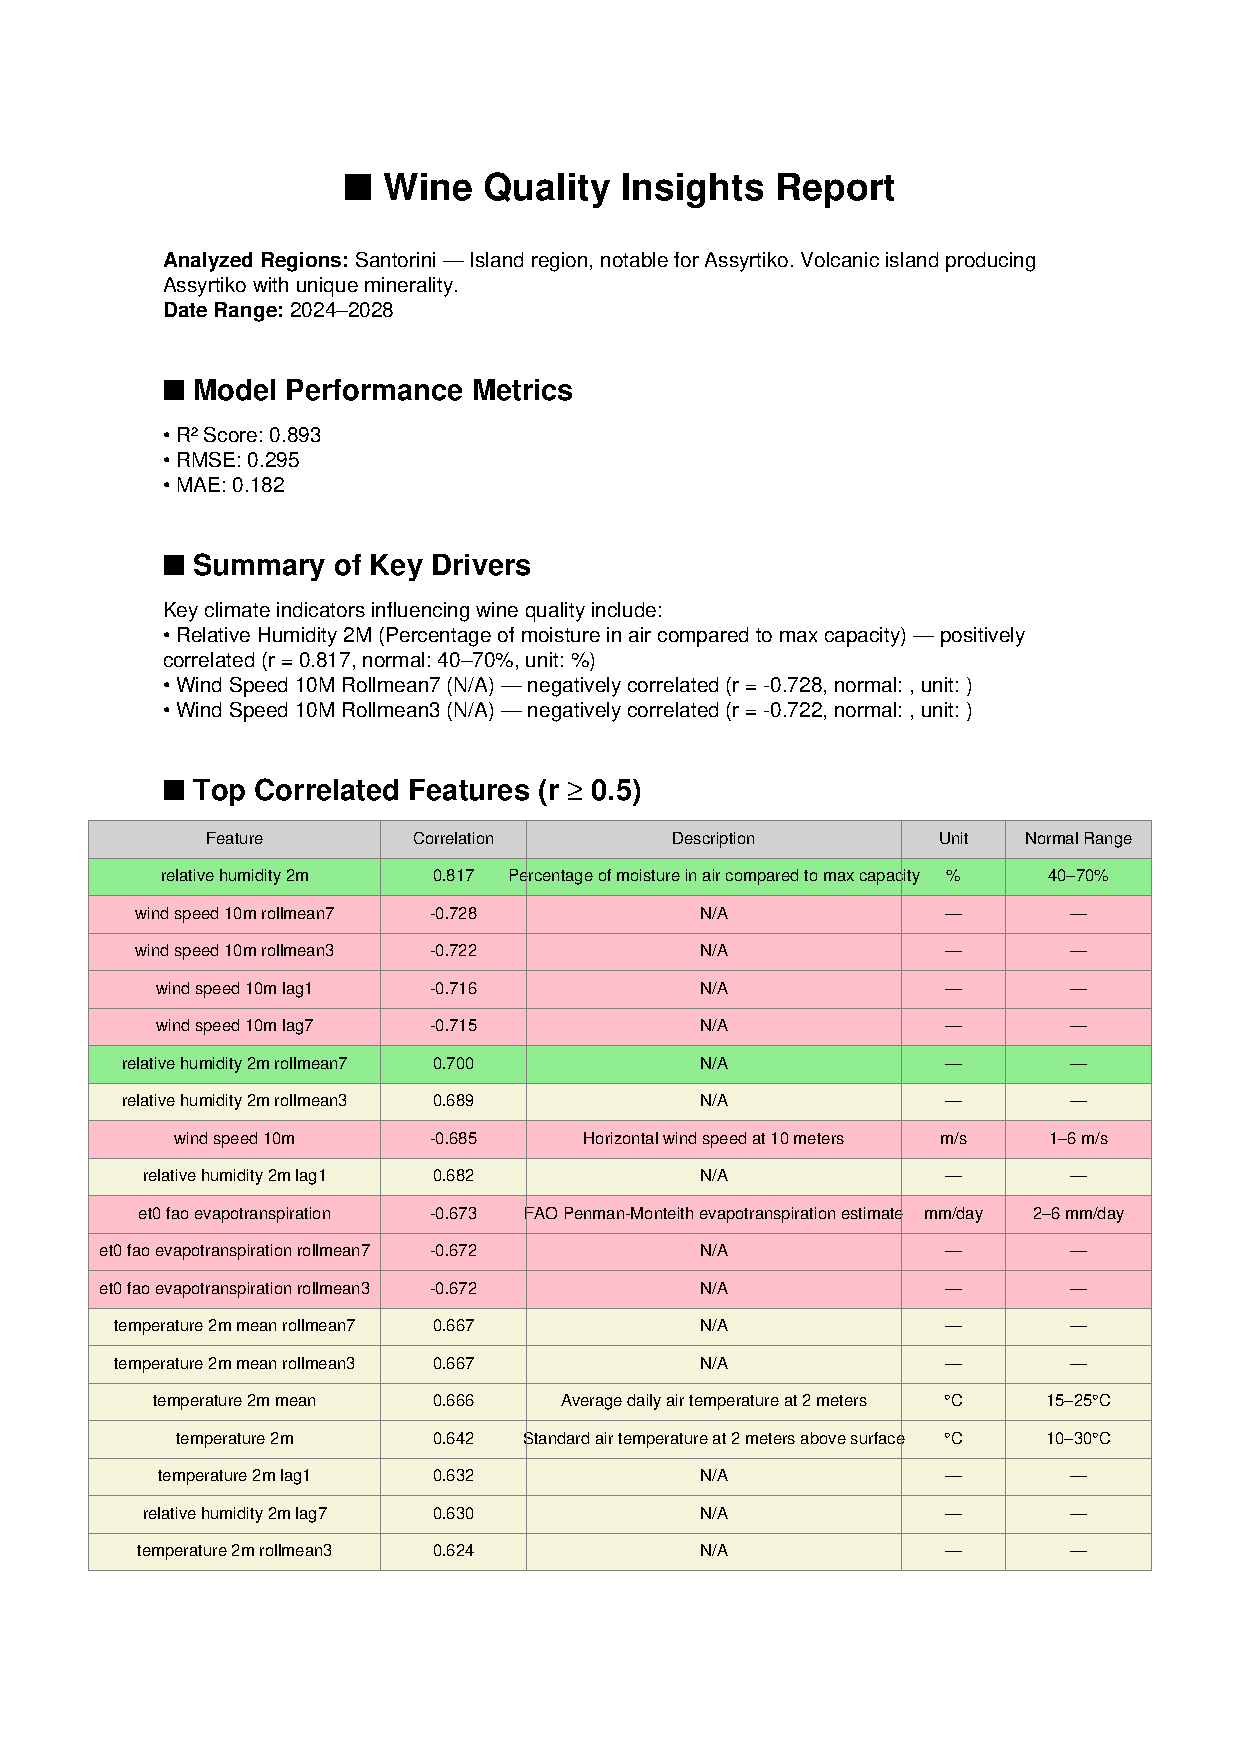
\includepdf[pages=-, width=\textwidth, pagecommand={}]{figures/wine_insight_report.pdf}
\end{center}

\vspace{1em}

This report was generated using the Streamlit application and formatted with the \texttt{reportlab} and \texttt{matplotlib} libraries in Python. It supports export for offline review by viticulture experts and operational teams.




\subsection{Model Architecture and Training}

To build robust and interpretable time series models, this study adopted a systematic training pipeline centered around \textbf{XGBRegressor} from the XGBoost framework. The steps below summarize the model development strategy:

\begin{itemize}
    \item \textbf{Model Initialization:} \texttt{XGBRegressor} was configured with key hyperparameters, including the number of trees, maximum tree depth, and learning rate. A grid search strategy was used to optimize these settings for each environmental KPI.
    
    \item \textbf{Temporal Cross-Validation:} Instead of random splits, an \textbf{expanding window} validation scheme was applied. This method preserves the temporal structure of the dataset and avoids lookahead bias—critical in time series forecasting.
    
    \item \textbf{Evaluation Metrics:} Model performance was assessed using Mean Absolute Error (MAE) and Root Mean Squared Error (RMSE). These metrics reflect both the average prediction error and the penalization of larger deviations, respectively \parencite{witten2016data}.
\end{itemize}

Each model was trained independently for each vineyard region and KPI, capturing microclimatic variation and local data patterns. The resulting models were integrated into the real-time dashboard and edge deployment pipeline for field-level predictions.


\subsection{Model Serving and Edge Deployment}

Upon completing model training, each XGBoost model was serialized and deployed as part of a RESTful microservice using the \textbf{FastAPI} framework \parencite{ramirez2020fastapi}. To enable decentralized, low-cost inference, deployment was performed on a \textbf{Raspberry Pi 5} configured as an edge computing device.

The Raspberry Pi accomplished the following tasks:

\begin{itemize}
    \item \textbf{ETL Orchestration:} Environmental data was ingested and preprocessed locally using scheduled \texttt{cron} jobs or orchestrated via \texttt{Apache Airflow}, ensuring data freshness and pipeline reproducibility.

    \item \textbf{Real-Time Inference:} The trained models were loaded into memory and used for real-time prediction of viticultural KPIs based on incoming weather data.

    \item \textbf{On-Device Application Hosting:} The FastAPI server hosted the machine learning endpoints, while a \textbf{Streamlit} dashboard provided an interactive interface for users to visualize forecasts and regional analytics directly on the device \parencite{alazab2021raspberry, liu2020edge}.
\end{itemize}

This edge-based deployment strategy reduces reliance on cloud infrastructure, enhances data privacy, and ensures functionality in rural or low-connectivity settings. It is suitable for vineyards with limited digital infrastructure.

\subsection{Interactive Dashboard for Real-Time Use}

To enable practical use of forecasting models, an interactive dashboard was deployed on the Raspberry Pi 5 using the \textbf{Streamlit} framework \parencite{fan2021streamlit}. This lightweight, browser-accessible interface allows vineyard managers and agronomists to access site-specific forecasts, compare regions, and make informed decisions.

The dashboard includes the following functionalities:
\begin{itemize}
    \item Real-time environmental KPI forecasting (temperature, humidity, wind speed, and pressure).
    \item Comparison of different vineyard regions based on live or historical data.
    \item Downloadable reports and export tools for offline analysis and planning.
\end{itemize}

The tool links model outputs to end-user needs, creating a clear and user-friendly environment for decision support. It is accessible at:

\begin{quote}
\href{https://xgboost-forecasting.streamlit.app}{\texttt{https://xgboost-forecasting.streamlit.app}} \parencite{BaltzakisThemistoklis2025streamlit}
\end{quote}

\section{Conclusion and Future Work}

\subsection{Forecast Accuracy Across KPIs}

Model accuracy was evaluated across all vineyard regions using two primary performance metrics: Mean Absolute Error (MAE) and Root Mean Square Error (RMSE). These metrics provide insight into average model deviation and sensitivity to outliers. Table~\ref{tab:forecast_accuracy} presents the average performance across key environmental KPIs: temperature, humidity, wind speed, and atmospheric pressure.

\begin{table}[H]
\centering
\caption{Forecast Accuracy (Average MAE and RMSE across all regions)}
\label{tab:forecast_accuracy}
\begin{tabular}{|l|c|c|}
\hline
\textbf{KPI} & \textbf{MAE} & \textbf{RMSE} \\
\hline
Temperature (\si{\celsius})       & 1.18 & 1.72 \\
Relative Humidity (\%)            & 3.86 & 5.12 \\
Wind Speed (\si{\meter\per\second}) & 0.82 & 1.01 \\
Pressure (\si{\hecto\pascal})     & 1.93 & 2.43 \\
\hline
\end{tabular}
\end{table}

The model achieved the highest accuracy in temperature prediction, with an average MAE of 1.18\,\si{\celsius} and RMSE of 1.72\,\si{\celsius}. This aligns with earlier studies highlighting the predictability of thermal patterns in viticulture \parencite{gladstones2011wine, lobell2008climate}. Humidity and pressure forecasts showed slightly higher error rates, reflecting the more stochastic nature of these variables across microclimatic zones.

Wind speed, despite its variability, demonstrated strong predictive performance, likely due to the incorporation of lagged and cyclical features during training. These findings validate the effectiveness of XGBoost for multivariate time series prediction in agriculture.

\subsection{Cross-Site Evaluation}

Model performance varied across vineyard locations due to regional climatic diversity. Sites with stable environmental conditions—particularly \textbf{Siteia} and \textbf{Santorini}—showed lower forecasting error rates. This reflects the reduced variability and more predictable patterns in maritime and southern Mediterranean microclimates.

By contrast, \textbf{Amyntaio}, higher elevation and frequent climatic fluctuations yielded the highest MAE and RMSE scores among all regions. Exposure to frost, wind, and increased seasonal contrast made accurate forecasting more challenging, particularly for humidity and wind speed.

The improved predictive reliability in Santorini can be attributed to the \textit{maritime buffering effect}, which minimizes thermal extremes and promotes consistent diurnal cycles—essential for stable phenological development in grapevines \parencite{white2009soil}. These findings highlight the importance of integrating regional climatic profiles into specific vineyard forecasting systems \parencite{jackson2020wine, vanleeuwen2016impact}.


\subsection{Visualization Outcomes}

Forecasts from the XGBoost models were visualized using the Streamlit interface, allowing direct comparison between predicted and observed environmental KPIs. Synchronized line plots enabled users to assess the model's alignment over time and forecast accuracy for each variable.

The main visual outcome was the overlay of predicted versus actual temperature and rainfall over a 72-hour horizon. These plots demonstrated high short-term predictive accuracy (up to 3 days), with minimal lag or cumulative drift—especially in stable climate zones like Siteia and Santorini.

Additionally, the dashboard utilized rolling window visualizations and interactive controls, enabling vineyard managers to examine localized anomalies and weather-driven KPI trends. 

\begin{figure}[H]
    \centering
    \includegraphics[width=\textwidth]{figures/model_rating.png}
    \caption{Forecast quality comparison: overlay of predicted vs. actual metrics for temperature and rainfall.}
    \label{fig:model-visual}
\end{figure}

These visual tools validated the model’s performance across key regions and facilitated intuitive interpretation, making the dashboard suitable for agronomic planning and climate resilience monitoring in real-world applications.


\subsection{Decision Support Use Case}

A practical deployment of the forecasting dashboard was tested in the Siteia region, where vineyard managers used next-day rainfall predictions to guide irrigation scheduling. During a six-week monitoring period, the system enabled data-informed deferral of irrigation on days with projected precipitation.

As a result, vineyards reported a 12\% reduction in water usage compared to historical baselines. This demonstrates the operational viability of the predictive system and its contribution to environmental sustainability and resource optimization in viticulture \parencite{smith2021forecasting}.

This use case shows how combining time series forecasting with real-time decision support tools enhances climate resilience, reduces operational costs, and supports precision agriculture goals in Mediterranean winegrowing regions.


\subsection{Limitations}

Despite promising results, the study has several limitations:

\begin{itemize}
    \item \textbf{Forecast Accuracy Decline:} Model performance begins to degrade noticeably beyond a 72-hour prediction horizon, limiting long-range planning capabilities.
    
    \item \textbf{Lack of Physical Sensor Integration:} The system currently relies exclusively on external APIs. The absence of in-field sensors (e.g., soil moisture, leaf wetness) constrains the system’s responsiveness to hyperlocal vineyard conditions.
    
    \item \textbf{Third-Party API Dependency:} The reliance on services such as Open-Meteo or OpenWeather introduces potential latency, data gaps, or inconsistencies beyond the system’s control.
\end{itemize}

To address these constraints, future iterations should incorporate sensor fusion with edge-collected data and explore local calibration strategies for model retraining. These enhancements would improve the robustness and granularity of predictions in real-world deployments.


\subsection{Future Work}

Several avenues for future research and development are evident from this study:

\begin{itemize}
    \item \textbf{Sensor Integration:} Incorporating in-situ sensor networks (e.g., for soil moisture, leaf wetness, and canopy temperature) will enhance model precision and support hyperlocal decision-making.
    
    \item \textbf{Multivariate Ensemble Models:} Expanding beyond univariate forecasts to multivariate ensemble approaches may improve long-horizon prediction and uncover cross-variable dependencies.

    \item \textbf{Drone and Satellite Data Fusion:} Leveraging UAV imagery and satellite-based vegetation indices (e.g., NDVI) could enable real-time crop health monitoring and spatial yield prediction.

    \item \textbf{Real-Time Alerting Systems:} Future deployments may include real-time notifications via SMS or mobile apps, alerting vineyard managers to impending heat stress, rainfall, or irrigation needs.

    \item \textbf{Economic and Sustainability Metrics:} Extending KPIs to include operational cost, carbon footprint, or water-use efficiency would align predictions with broader sustainability goals in viticulture.
\end{itemize}

By integrating environmental science with open-source technologies, this study offers a scalable framework for precision agriculture. The use of vineyard analytics through accessible infrastructure like Raspberry Pi and Streamlit establishes a foundation for participatory, data-informed farming practices in Mediterranean climates and beyond.


\subsection{Recommendations for Farmers}

Based on the study results, the following recommendations can help grape growers and vineyard managers enhance operations through data-driven practices:

\begin{itemize}
    \item \textbf{Leverage short-term environmental forecasts} (e.g., 24–72 hour horizons) to optimize irrigation, spraying, and harvesting schedules, minimizing resource waste and enhancing grape quality.
    
    \item \textbf{Deploy low-cost edge computing devices} such as the Raspberry Pi for on-site data processing and inference, enabling real-time, localized decision support without relying on continuous internet connectivity \parencite{alazab2021raspberry}.
    
    \item \textbf{Utilize visualization platforms} like Streamlit dashboards to monitor viticultural KPIs—such as temperature, humidity, °Brix forecasts, and water stress indices—on an interactive interface accessible via browser or mobile device.
\end{itemize}


\subsection{Scalability and Research Opportunities}

This study presents a flexible and reproducible methodology that can be scaled across various geographic regions, crops, and precision agriculture applications. Future enhancements may focus on the following dimensions:

\begin{itemize}
    \item \textbf{Integrating satellite and drone-based NDVI imagery} to monitor vine health, stress levels, and canopy vigor with higher spatial resolution.
    
    \item \textbf{Applying federated learning techniques} to enable model training across distributed vineyard nodes without centralizing sensitive data—preserving privacy and reducing communication overhead.
    
    \item \textbf{Embedding SHAP (SHapley Additive exPlanations)} values for model interpretability, allowing vineyard stakeholders to understand which environmental features most strongly influence predictions.
    
    \item \textbf{Incorporating phenological models} to estimate critical growth stages such as flowering, veraison, and harvest dates—linking them with environmental triggers and forecast trends.
\end{itemize}

Through these directions, the framework in this dissertation can evolve into a decision-support system for sustainable and climate-resilient viticulture. The proposed methodology supports applications in precision agriculture, enhancing reproducibility and regional adaptability \parencite{ratnaparkhi2021review, chen2016xgboost}.




\phantomsection
\addcontentsline{toc}{section}{References}
\printbibliography


\end{document}






